% Name: F-move, time going down
% Description: The same F-move read from top to bottom: d at the top splits into a, b, and c below, with the same coefficient [F^{abc}_d]_{ef}.
% Tags: F-move, F-symbol, associativity, fusion category, time going down

$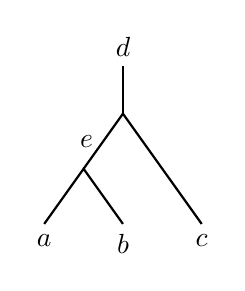
\begin{tikzpicture}[thick, baseline=(current bounding box.center)]
  \draw (0,0) node[below] {$a$} -- (0.5,0.7) -- (1,0) node[below] {$b$};
  \draw (0.5,0.7) -- node[left] {$e$} (1,1.4) -- (2,0) node[below] {$c$};
  \draw (1,1.4) -- (1,2) node[above] {$d$};
\end{tikzpicture}
\;=\; \sum_f \bigl[F^{abc}_d\bigr]_{ef}
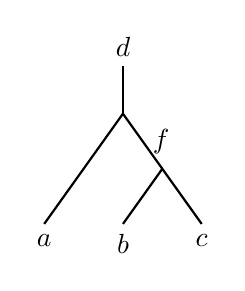
\begin{tikzpicture}[thick, baseline=(current bounding box.center)]
  \draw (0,0) node[below] {$a$} -- (1,1.4);
  \draw (1,0) node[below] {$b$} -- (1.5,0.7) -- (2,0) node[below] {$c$};
  \draw (1.5,0.7) -- node[right] {$f$} (1,1.4);
  \draw (1,1.4) -- (1,2) node[above] {$d$};
\end{tikzpicture}$
